
\chapter{Double twisted membranes versus ribbons in colloidal rods stabilized by polymer depletion}
\chaptermark{Tactoid morphology}



\begin{abstract}

At the mesoscopic level, rigid rodlike colloids with chiral features such as {\rm fd} virus rods mixed with non-adsorbing polymer form a variety of different liquiod crystalline droplets with varying shape and internal twisted structure. Inspired by recent experiment work on the droplet morphology of these rod-polymer mixtures, we use extensive Monte Carlo simulations supplemented with theory to explore two prominent droplet shapes, namely the double twisted membrane and the twisted ribbon. In experiment, the elongated ribbon structure is found to dominate at elevated chiral strength. In our simulations, however, we demonstrate that upon increasing chirality the membranes tend to transition into multi-domain structures consisting of multiple double-twisted near-circular units separated by $\pi$-walls, while the transition into twisted ribbons appears impeded for reasons unknown.  We also briefly discuss the role of planar confinement on the droplet morphology  in relation to recent experimental work on {\em fd}-polymer mixtures.

\end{abstract}



\section{Introduction}




Rodlike colloidal particles are capable of assembling into a variety of liquid crystalline mesostructures whose bulk properties depend primarily on the topology of the director field indicating the average direction of rod alignment \cite{dogic-fraden_fil,Ikkala2407}.
In general,  site-specific attractive forces between non-spherical nanoparticles may affect the self-assembly properties  and lead to a wealth of different superstructures \cite{Wang358} such as twisted ribbons of semi-conducting rods \cite{Srivastava1355} or platelets \cite{Janae1701483}.
Mixing rodlike colloids with non-adsorbing polymers or other small depletant particles induces a short-ranged attractive  (`sticky') effective potential between the rods that can be exploited to control the self-assemby morphology \cite{Baranov2010,Sharma2014}. 
 


 The size and concentration of the added polymer can be exploited to  tune the morphology and internal structure of the droplets. Tactoids with nematic-type order have been observed experimentally in mixtures of rods and big depletants (typically bigger than the diameter of the colloidal rods), as well as smectic-like single layer droplets, named colloidal membranes, when significantly increasing polymer concentration. The morphology of these membranes is further controlled by strong electrostatic and chiral twist interactions between the individual rods. Though these interactions are not well understood yet, it has been empirically observed that, in close contact with one another, {\em fd} rods tend to twist preferentially clockwise, instead of arrange following a global nematic direction. When both depletion effect and chirality are strong, double-twisted colloidal membranes tend to destabilize to give way to twisted ribbons. The additional effect of intrinsic particle chirality
strongly impinges  onto the self-assembled mesostructure and drives a vast range of different twisted or chiral structures ranging from smectic membranes to chiral ribbons  \cite{Gibaud2014} and hexagonal nanocrystals displaying screw-dislocations \cite{grelet1}. These twisted structures have been observed experimentally, but reproducing these structures in computer simulation has been elusive so far. 



Further complexity can be achieved by the presence of strong geometric confinement.  In this study we will consider a slab geometry with width comparable to the rod length. The confinement is expected to generate tactoids with a strongly non-uniform rod density whose morphology is further controlled by a surface tension that strongly depends on the average rod orientation with respect to the surface normal. In fact, the presence of the wall imparts a wall-liquid surface tension which is likely to be different from the liquid-gas surface tension which would dominate in the bulk case.

We study these systems (both in bulk and under narrow confinement) by means of Monte Carlo simulations in the semi-grand canonical ensemble ($N,V,\mu_{p},T$) consisting of a system of $N$ rods in a volume $V$ at constant temperature $T$ in osmotic equilibrium with a polymer reservoir at constant chemical potential $\mu_{p}$. The number of polymers  $N_{p}$ in the system is then a fluctuating quantity with the average polymer concentration controlled by $\mu_{p}$.

\section{Model and simulations}

We consider a system of $N$ rigid spherocylinders of length $L$, thickness $D$ and aspect ratio \red{$L/D = 10$ or $20$}. The spherocylinders are a simplified representation of {\em fd} rods that are much thinner ($L/D > 100$) and carry a small degree of backbone flexibility with persistence length $\ell_{p} \gg L$. Since the large particle aspect ratio in combination with backbone flexibility poses considerable limitations on the numerical efficiency of our simulations  we  only consider rigid rods with a relatively short length assuming that the key features of the mesoscopic structures evaluated in this work do not  critically depend on the rod aspect ratio or flexibility.

The spherocylinders are mixed with non-adsorbing polymers that in our model act as non-penetrable hard spheres with diameter $\sigma$ equalling once or twice that of the spherocylinder ($\sigma = D$ or $2D$). Polymer-polymer interactions are zero, while the interaction between a polymer and a spherocylinder are treated as being strictly hard;  the potential energy is infinitely large when a  sphere and spherocylinder overlap and zero otherwise.



\begin{figure}
	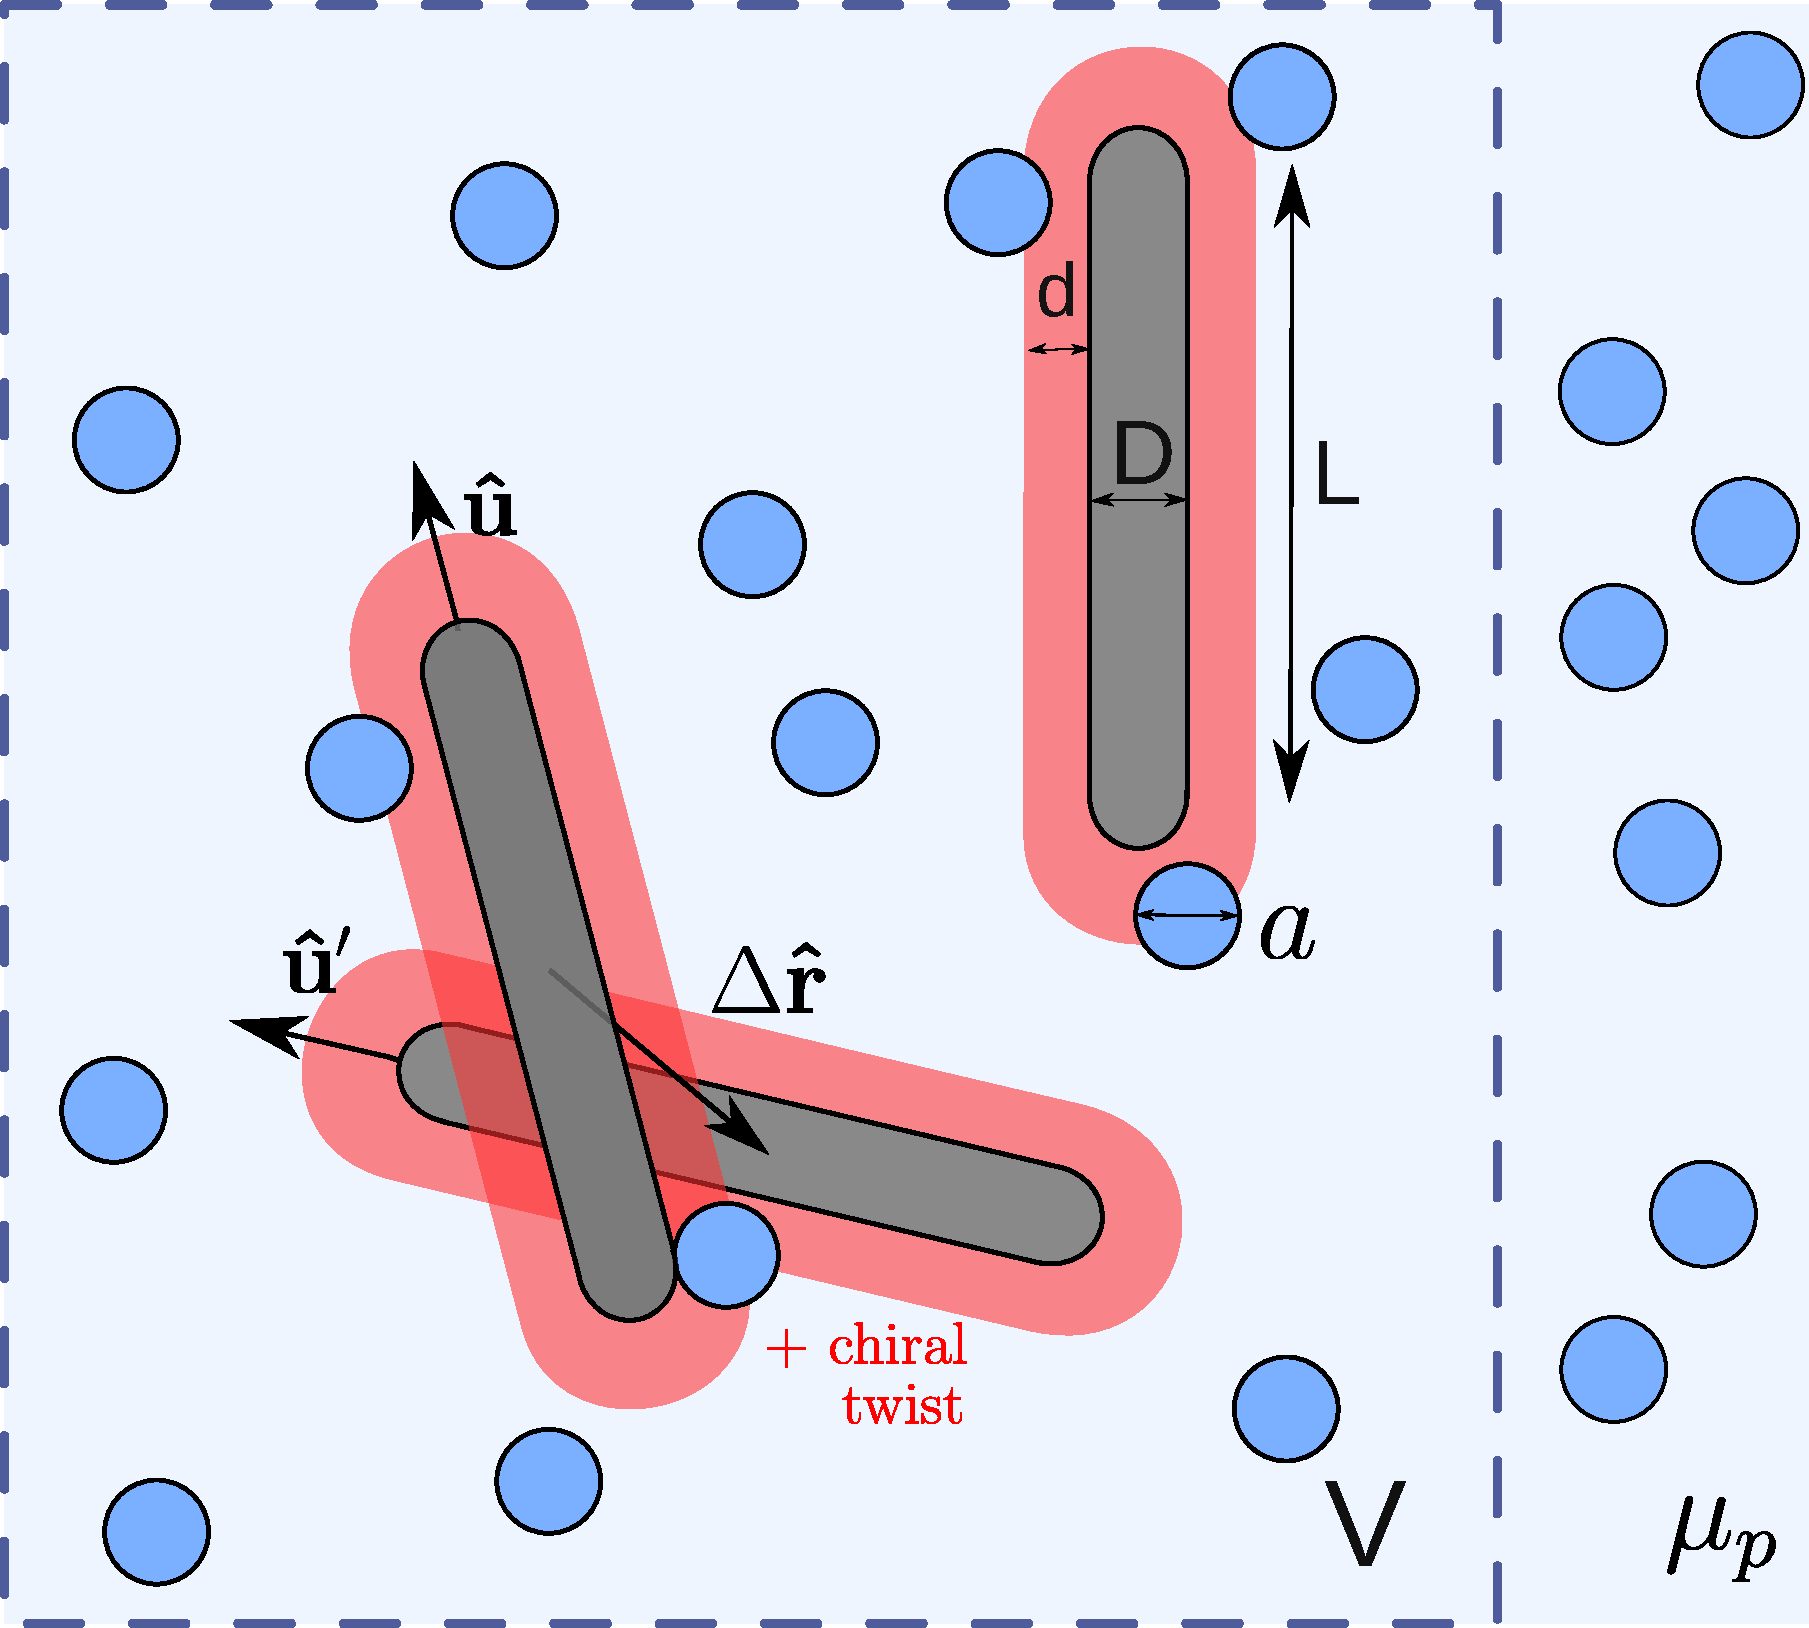
\includegraphics[width = \columnwidth]{figures/chapter-5/spheromans}
	\caption{ Sketch of the simulation model: hard spherocylinders (grey) mixed non-penetrable polymers (blue) with diameter $\sigma = D$ (as depicted here). Overlap of the cores (grey) gives infinite repulsion while overlapping coronae (blurred zones) favors a twisted pair configuration representing the (chiral) electrostatic forces between {\em fd} rods. Two possible setups are considered: (a) The system is in an unconfined environment under periodic boundary conditions. (b) The system is confined in a slab geometry with wall-to-wall distance $h$. Note that this model is defined in (a) two or (b) three spatial dimensions. }
	\label{sketch}
\end{figure}


\subsection{Chiral interactions}

The pair interaction $U_{r}$ between two spherocylinders with solid angles $\oma$ and $\omb$ and centre-of-mass distance $\Delta \bfr$ follows from a combination of short-range steric forces (treated as strictly hard) and electrostatic forces at larger distance. The  interaction potential between a pair rods depends on centre-of-mass distance vector $\Delta {\bf r}$ and orientation vector $\oma$ of both rods. In our model, the interactions are encapsulated in the following core-shell potential:
\beq
U_{\rm r} (\Delta {\bf r}, \oma, \omb) =
\begin{cases}
\infty & \textrm{if hard cores overlap}\\
U_{\rm twist} & \textrm{otherwise} \\
\end{cases}
\label{urod}
\eeq
The electrostatic interactions between {\em fd} rods gives rise to so-called electrostatic twist which is intimately linked to the chirality surface architecture of {\em fd} virus rods. The chiral  potential is commonly expressed in terms of a pseudoscalar form initially put forward by Goossens: % TODO: reference Goossens
\beq
U_{\rm twist} (\Delta {\bf r}, \oma , \omb )=
-\varepsilon_{c} \left ( \frac{D}{\Delta r} \right )^{7}(\oma \cdot \omb)(\oma \times \omb \cdot \Delta \hat{\bf r})
\eeq
where  $\Delta \hat{\bf r} $ denotes a unit vector for the centre-of-mass distance.
 The sign of $\varepsilon_{c}$ defines the microscopic handedness of the rods. Without loss of generality we take $\varepsilon_{c} > 0$ reflecting the right-handedness of {\em fd} rods. The chiral symmetry of the potential is expressed by the pseudoscalar that imparts a sign change upon  inversion $\Delta \hat{\bf r} \rightarrow - \Delta \hat{\bf r}$. In view of its rapid decay with $\Delta r$ the potential is very short-ranged and the rods need to be very close together in order to feel the chiral twist.

 %For simplicity, we assume that the twisting forces are sufficiently short-ranged (which should be the case at sufficient ionic strength) and do not  continuously vary with the centre-of-mass distance between the spherocylinders, but are only operative if the coronae between the rods overlap (see \fig{sketch}).

\subsection{Estimation of the depletion strength for two parallel spherocylinders}

 The typical attraction energy between two rods due to polymer depletion can be estimated from free-volume theory \cite{lekkerkerker2011depletion} and reads:
 \beq
 U_{\rm r,dep} \sim -\Pi_{P} V_{\rm r, ov}
 \eeq
with $ \Pi_{P} = k_{B} T N_{P}/V$ the (van't Hoff) osmotic pressure of the polymer reservoir and $V_{\rm r, ov}$ the overlap volume  of the depletion layers surrounding each rod which depends on the orientation of each rod. In case the rods are perfectly parallel and at hard-core contact we find a simple analytical result. Ignoring  finite rod size effects we have:
\beq
V_{\rm r, ov} = LD^{2} \left [  2 r^{2} \cos^{-1} \left ( \tfrac{1}{2r} \right )  - \tfrac{1}{2} \sqrt{4 r^{2} -1}  \right ]
\eeq
with $r = \tfrac{1}{2}(1 + \tfrac{\sigma}{D})$. Rescaling in terms of the polymer packing fraction in the reservoir we find that the maximum depletion strength per rod pair  reads:
\beq
  U_{\rm r,dep} \sim - k_{B}T \phi_{P}  \frac{L}{D} \left ( \frac{D}{\sigma} \right )^{3} \left [  2 r^{2} \cos^{-1} \left ( \tfrac{1}{2r} \right )  - \tfrac{1}{2} \sqrt{4 r^{2} -1} \right ]
 \eeq
For a typical set-up ($\phi_{P} =3$, $\sigma = 2D$ and $L/D=10$) this gives about 15 $k_{B}T$ \red{Please verify this}.

A key parameter in this system is the relative strength of chiral twist versus depletion attraction. These can be combined into a dimensionless parameter $\chi_{T}$ balancing the energy scales associated with twist and depletion as previously discussed:
\beq
\chi_{T} = \frac{\varepsilon_{c}}{U_{\rm r, dep}} \ll 1
\eeq
so that twist becomes more prevalent for larger $\chi_{T}$. It is important to keep in mind that the typical energy due to chiral twist should be small ($ | \varepsilon_{c} | \ll U_{\rm r,dep} $) in order to ensure that the cohesive forces among the rods residing in a droplet are dominated by polymer depletion, with chiral twist playing only a perturbative role.

\subsection{Semi-grand canonical ensemble}
% TODO: change this section to add Glaser's Algorithm

The simulations are carried out in the semi-grand ensemble, with a fixed number of rods but the polymer content in the system fluctuating against a virtual reservoir consisting of an ideal gas of polymer spheres with a prescribed chemical potential  $\mu_{p}$ which is trivially connected to the polymer packing fraction via:
\beq
\phi_{P} = \frac{\pi D^{3}}{ 6 \Lambda_{p}^{3} } e^{\beta \mu_{P}}
\eeq
where $\Lambda_{P}$ denotes the thermal (de Broglie) wavelength.

\subsubsection{Version I: Explicit depletants}

Each MC cycle consists of $N + N_{P}$ randomly chosen rod translations, rotations, polymer insertions or removals.

\subsubsection{Version II: Implicit depletants}

\red{Here we need to specify Glaser's cluster move optimization algorithm that we used \cite{glaser2015parallel}.}

\subsection{Rod-wall interactions}

One possible variation of our model is to confine the rods and polymers in a thin slab of width $h = L$ (see \fig{sketch}). The wall-spherocylinder interactions  are strictly hard, that is, infinite repulsion when the spherocylinder core overlaps with the wall and zero repulsion otherwise. More specifically:
\beq
U_{\rm w} (\Delta {\bf r}, \oma) =
\begin{cases}
\infty &  | \Delta {\bf r} \cdot {\bf \hat{n}} | < \frac{L}{2}  | \oma \cdot {\bf \hat{n}} | + \tfrac{D}{2} \\
\infty &   h-  | \Delta {\bf r} \cdot {\bf \hat{n}} | < \frac{L}{2}  | \oma \cdot {\bf \hat{n}} | + \tfrac{D}{2} \\
0 & \textrm{otherwise}
\end{cases}
\label{urodwall}
\eeq
with ${\bf \hat{n} }$ denoting the wall normal.

Polymers are not allowed to overlap with the wall. However, another parameter of the system is the wall depletion range $\sigma_W$ that will take values typically lower than $\sigma$. This strategy is aimed to tune the amount of wetting felt by the tactoids close to the wall, allowing equilibration of partial wetting scenarios. A physical argument for this reduction of the wall depletion range (that in principle would only depend on the size of the depletants), is the variation of the electrostatic forces affecting superficial charges both around the rods and the wall, that may change the effective size of the depletion regions unfavorable for the non-adsorbing polymers. % TODO: cite, verify!!
%The polymers do not have any interaction with the wall, but their centres-of-mass are constrained  to reside within the slab.

\subsection{Simulation} % TODO: change this title??

Monte Carlo simulations are performed for different scenarios conceived from the specifications of the previous sections.

The step size for the spherocylinder translations and rotations are chosen adaptively such as to maintain an average acceptance ratio of about 30 \%. The MC code is optimized using cell-linked list routines that significantly reduce the number of overlap checks between rod-rod and rod-polymer pairs involved in  each MC step. We keep a rectangular box shape with $L_{x} = L_{y}$ and $L_{z} = h = L$ and periodic boundary conditions (PBC) in both lateral directions.

%Depending on the polymer size and concentration the system will either evolve into a liquid drop ("tactoid") or  will retain its crystalline inner structure (expected for `sticky' depletion forces induced by small polymers, $\sigma = D$).
We monitor the total overlap volume of the depletion layers $V_{\rm T, ov}$ and the total twist energy $\mathcal{U}  = \sum_{i}\sum_{j<i}U_{\rm twist}$ to gauge whether the drop has reached its equilibrium state.

We plan to focus on two different systems:

\begin{itemize}
\item  Small polymers with $\sigma = D$ imparting short-ranged attractions. The initial configuration is a square monolayer of perfectly parallel rods ordered into a hexagonal lattice. Without confinement, the cluster will equilibrate into a membrane with  fluid order. In. our simulations we fix the polymer concentrations $\phi_{P}=1$ and $N=2000$. Note that small changes in $\epsilon_{c}$ may have large consequences for the way the droplet expresses chiral twist. At weak twist ($\varepsilon_{c} < ****$), the membrane remains circular in shape with twist showing up at the membrane edges while the membrane center remains largely unperturbed. At strong twist ($\varepsilon > ****$) the membrane may transform into a twisted ribbon. \red{The first indication of such a change of droplet morphology can be observed in \fig{samples} a and c.   Bigger systems ($N=2000$) spontaneously form ribbon-shaped protrusions around a circular central body which resembles the onset of twisted ribbon formation.  }.  Next we introduce confinement and re-assess the droplet shape and internal structure and compare with experimental observations.

\item Large polymers with $\sigma = 2 D$ imparting long-ranged attractions. We start from the same monolayer crystal which will equilibrate into a liquid tactoid in bulk \cite{kuhnhold2022structure}. Gradually increasing the confinement (at $R_{2} > h$ with $R_{2}$ the minor curvature radius of an unconfined tactoid \cite{kuhnhold2022structure})  will lead to squeezed tactoids which  develop a distinct biaxial shape. Introducing twist may lead to further morphological changes. We may correlate droplet size ($N$) with droplet aspect ratio for the strongly confined case compared to the 3D case studied in \cite{kuhnhold2022structure}.

\end{itemize}

%\begin{itemize}
%\item  Small polymers with $\sigma = D$ imparting short-ranged attractions. The initial configuration is a square monolayer of perfectly parallel rods ordered into a hexagonal lattice. Without confinement, the cluster will equilibrate into a membrane with  fluid order. In. our simulations we fix the polymer concentrations $\phi_{P}=1$ and $N=2000$. Note that small changes in $\epsilon_{c}$ may have large consequences for the way the droplet expresses chiral twist. At weak twist ($\varepsilon_{c} < ****$), the membrane remains circular in shape with twist showing up at the membrane edges while the membrane center remains largely unperturbed. At strong twist ($\varepsilon > ****$) the membrane may transform into a twisted ribbon. \red{The first indication of such a change of droplet morphology can be observed in \fig{samples} a and c.   Bigger systems ($N=2000$) spontaneously form ribbon-shaped protrusions around a circular central body which resembles the onset of twisted ribbon formation.  }.  Next we introduce confinement and re-assess the droplet shape and internal structure and compare with experimental observations.
%
%\item Large polymers with $\sigma = 2 D$ imparting long-ranged attractions. We start from the same monolayer crystal which will equilibrate into a liquid tactoid in bulk \cite{kuhnhold2022structure}. Gradually increasing the confinement (at $R_{2} > h$ with $R_{2}$ the minor curvature radius of an unconfined tactoid \cite{kuhnhold2022structure})  will lead to squeezed tactoids which  develop a distinct biaxial shape. Introducing twist may lead to further morphological changes. We may correlate droplet size ($N$) with droplet aspect ratio for the strongly confined case compared to the 3D case studied in \cite{kuhnhold2022structure}.
%
%\end{itemize}

\section{Results}

\begin{figure}
	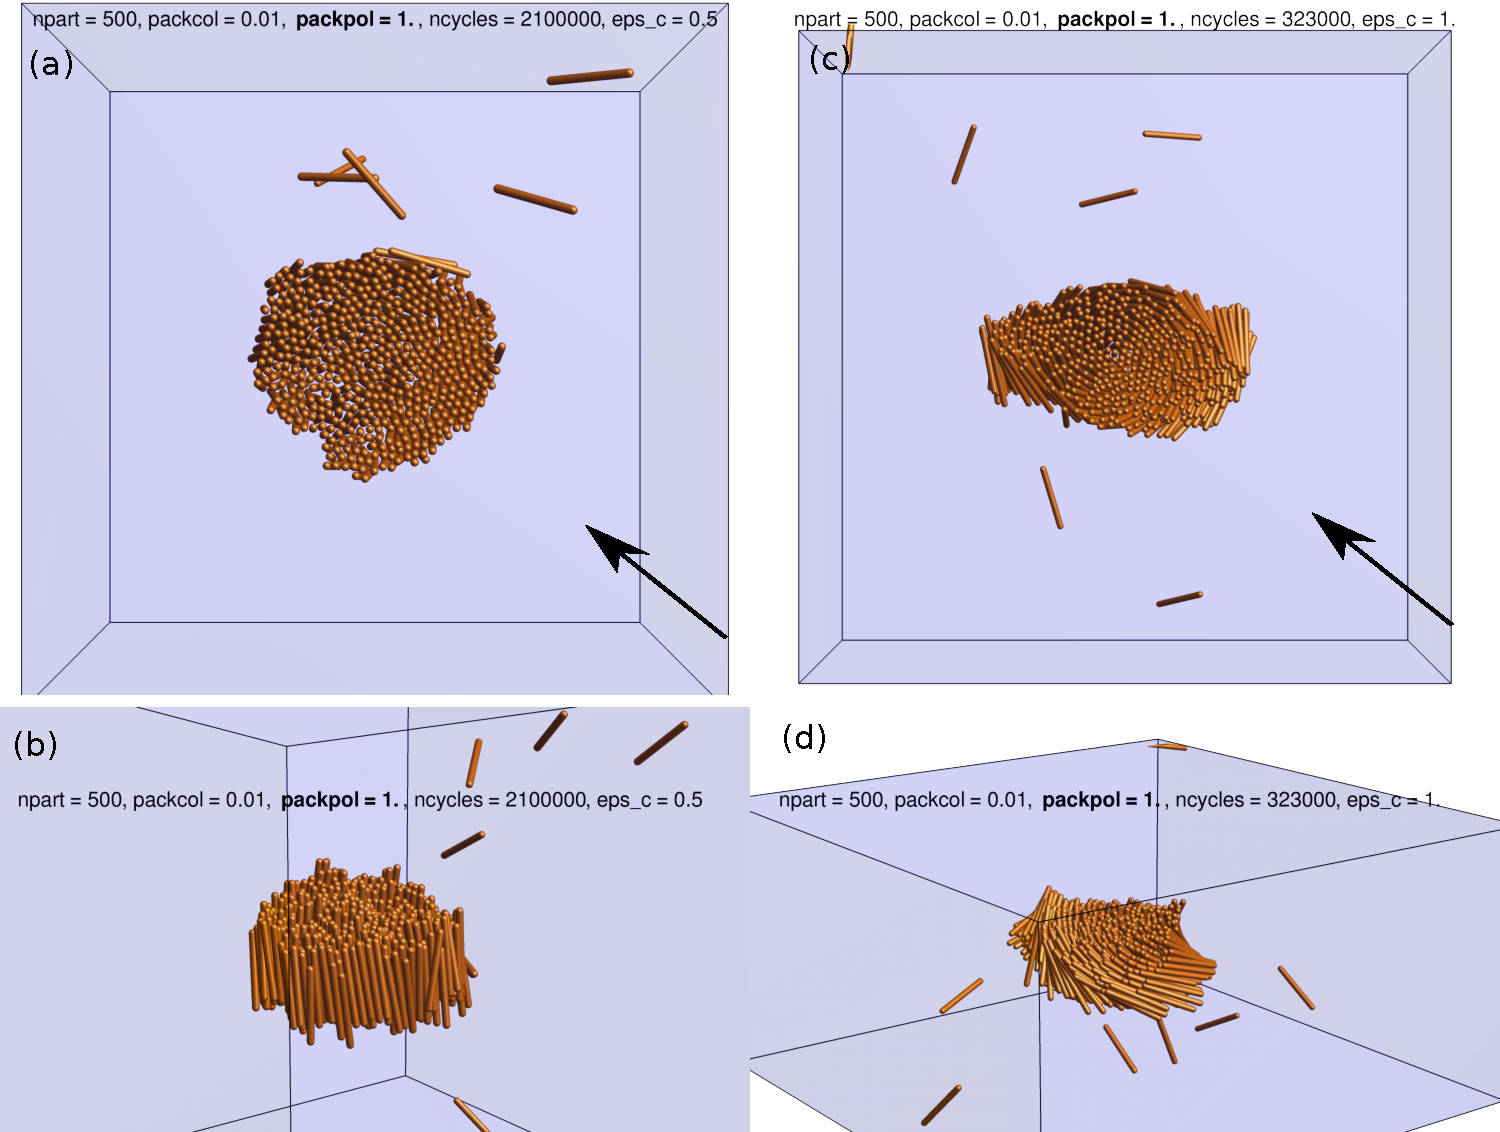
\includegraphics[width = .7\columnwidth]{figures/chapter-5/samples}
	\caption{Membrane-shaped tactoids of chiral rods mixed with non-adsorbing polymer formed in bulk (no confinement). For all runs, $\sigma = D$, chiral radius $d = 0.4D$, $\phi_{P}$ and $N = 500$. (a)-(b) $\varepsilon_{c}=0.5k_BT$, (c)-(d) $\varepsilon_{c}=1k_BT$ Top panels (a),(c) correspond to a top view of the system, bottom panels (b), (d) correspond to a side view with angle indicated by an arrow at the top panels.}
	\label{samples}
\end{figure}

\begin{figure}
	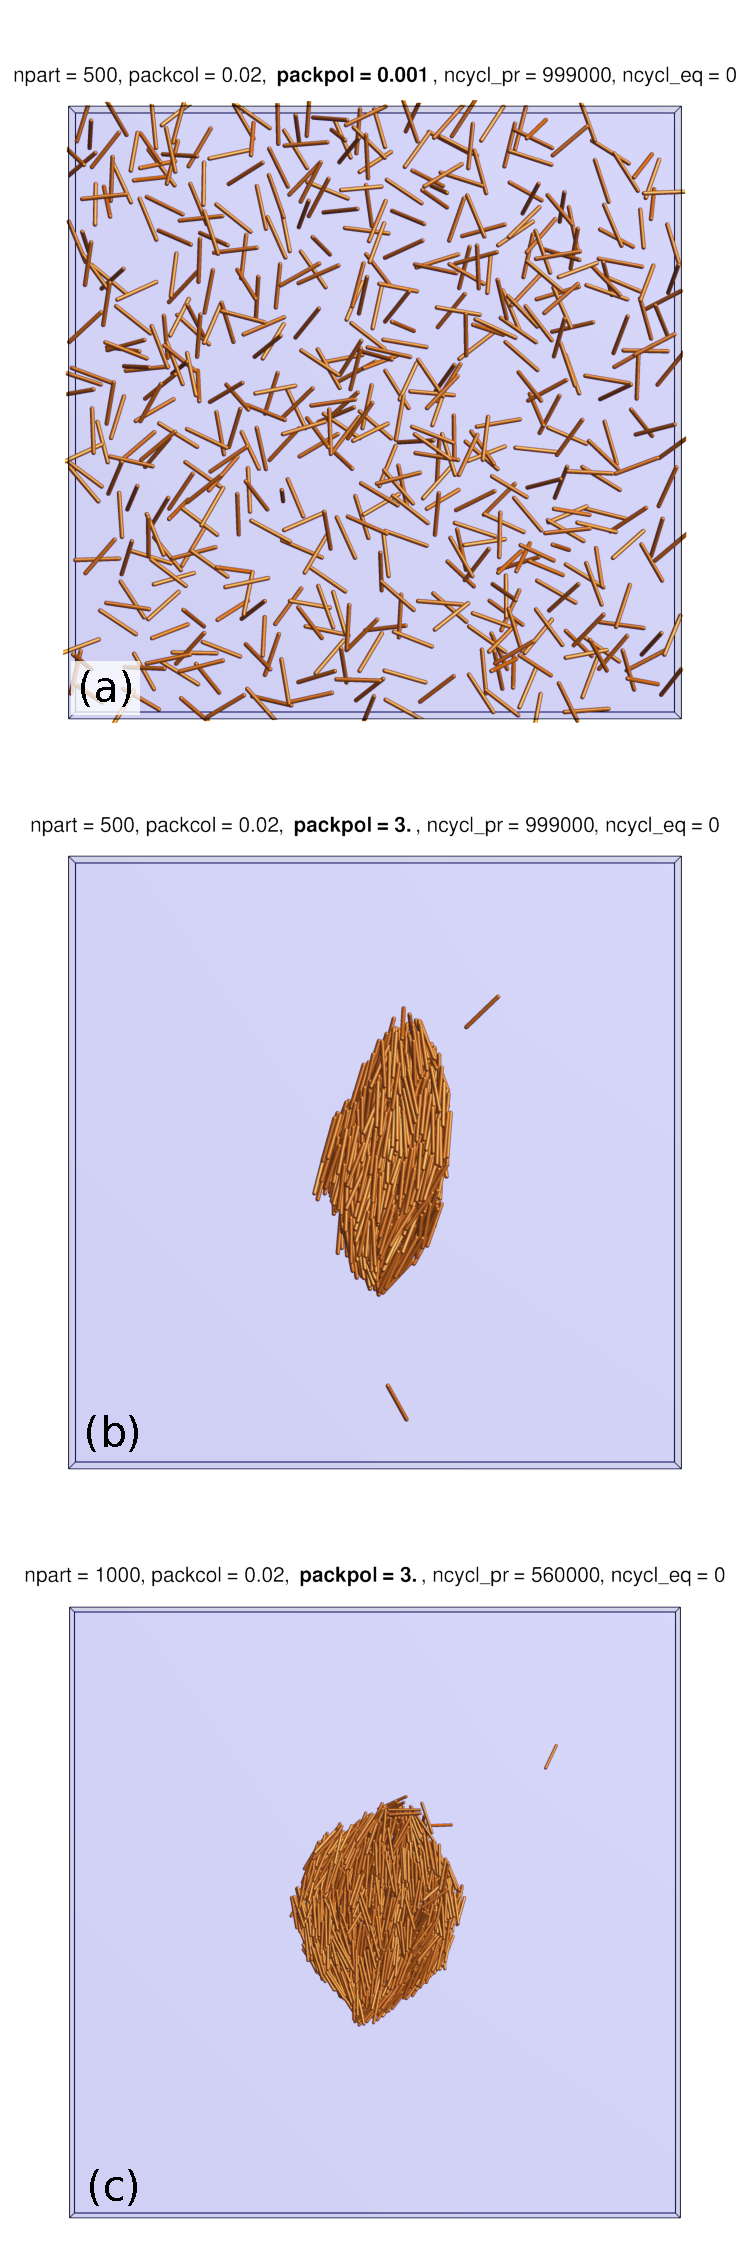
\includegraphics[width = 0.4 \columnwidth]{figures/chapter-5/impl_depletion_effect}
	\caption[Spindle-shaped tactoids of achiral rods mixed with non-adsorbing polymer \red{in strong planar confinement}]{ Spindle-shaped tactoids of achiral rods ($\varepsilon_{c}=0$) mixed with non-adsorbing polymer ($\sigma = 2D$) \red{in strong planar confinement ($h = L+D$)}. a) Weak depletion  (very low polymer packing fraction) and $N=500$. b) Strong depletion; $\phi_{P} =3$, $N=500$. c) Strong depletion; $\phi_{P} =3$, $N=1000$. The difference between the shapes between (b) and (c) is explained in \cite{kuhnhold2022structure} for 3-dimensional tactoids: larger nematic droplets tend to be less elongated. The structure in panel (b) is used as an initial configuration in the samples shown in \fig{samples}}
	\label{notwist}
\end{figure}






\section{Theory for double-twisted membranes}

 To complement our simulations results we now develop a theory for double-twisted membranes by focussing on two distinct morphologies that have been observed in experiment, namely half-skyrmion-type membranes and twisted ribbons. 
 Let us begin by recalling the well-known Frank-Oseen elastic energy of the general case of a bulk chiral liquid crystal for and arbitrary nematic director field $\bn$ in three spatial dimensions:
\begin{align} 
F = & \frac{1}{2} \int d \bfr \left [ K_{1} (\nabla \cdot \bn)^{2}  + K_{2} (\bn \cdot \nabla \times \bn + q_{0})^{2}  +   K_{3} (\bn \times \nabla \times \bn)^{2} \right ]  
\end{align}
with $K_{1}$, $K_{2}$ and $K_{3}$ respectively denoting the splay, twist and bend elastic moduli.   The inverse  pitch  $q_{0}$ quantifies the chiral strength of the particles in the liquid crystal. 


 For the specific case of a cylindrically symmetric, double-twisted membrane depicted in\fig{memsnap}
  with radius $R_{m}$ we may invoke a cylindrical geometry  with radial coordinate $0<R< R_{m}$ and angle $\alpha$.  Deformations from a uniform director field in which case $\bn = \bz$ are assumed to be concentric and can be described as:
 \beq
 \bn = \cos \psi (R) \cos  \varphi(R) \bz + \cos \psi (R) \sin \varphi(R) \bal + \sin \psi(R) \bars
 \label{tilt}
 \eeq
in terms of a twist angle  $ \varphi $ denoting a twist deflection of the rods with respect to the membrane normal and $\psi$ a splay deformation along the membrane radial vector (see \fig{memsnap}).   We the local rod density within the membrane to be uniform so that the one-body density reads $\rho(R, \bw)  = \rho_{0}f(R,  \bw)$, in terms of the rod number density $\rho_{0}$ denoting the number of rods per area unit, and a three-dimensional rod unit vector $\bw$ distributed along the local director obeying an a priori unknown distribution $f$. The twist-bend elastic free energy  takes the following form \cite{barry_jpcb2009,wensink2018elastic}:
\begin{align}
 F_{el}  &= \int  d \brr \left [ K_{2} \left ( \partial_{R} \varphi + \frac{\sin 2 \varphi}{2R} + q_{0} \right )^{2}  + K_{3}\frac{ ( \sin \varphi )^{4}}{R^{2}} \right   ]
\label{fmem}
\end{align}
with $\int d {\bf R} = 2 \pi \int_{0}^{R_{m}} R dR $ in circular coordinates for a membrane with radius $R_{m}$.
 The  elastic moduli for the membrane are distinctly different from those of a ulk liquid crystal and will be specified in the next section. We remark that these elastic moduli are strictly 2D quantities with dimension energy.  



\begin{figure}
\begin{center}
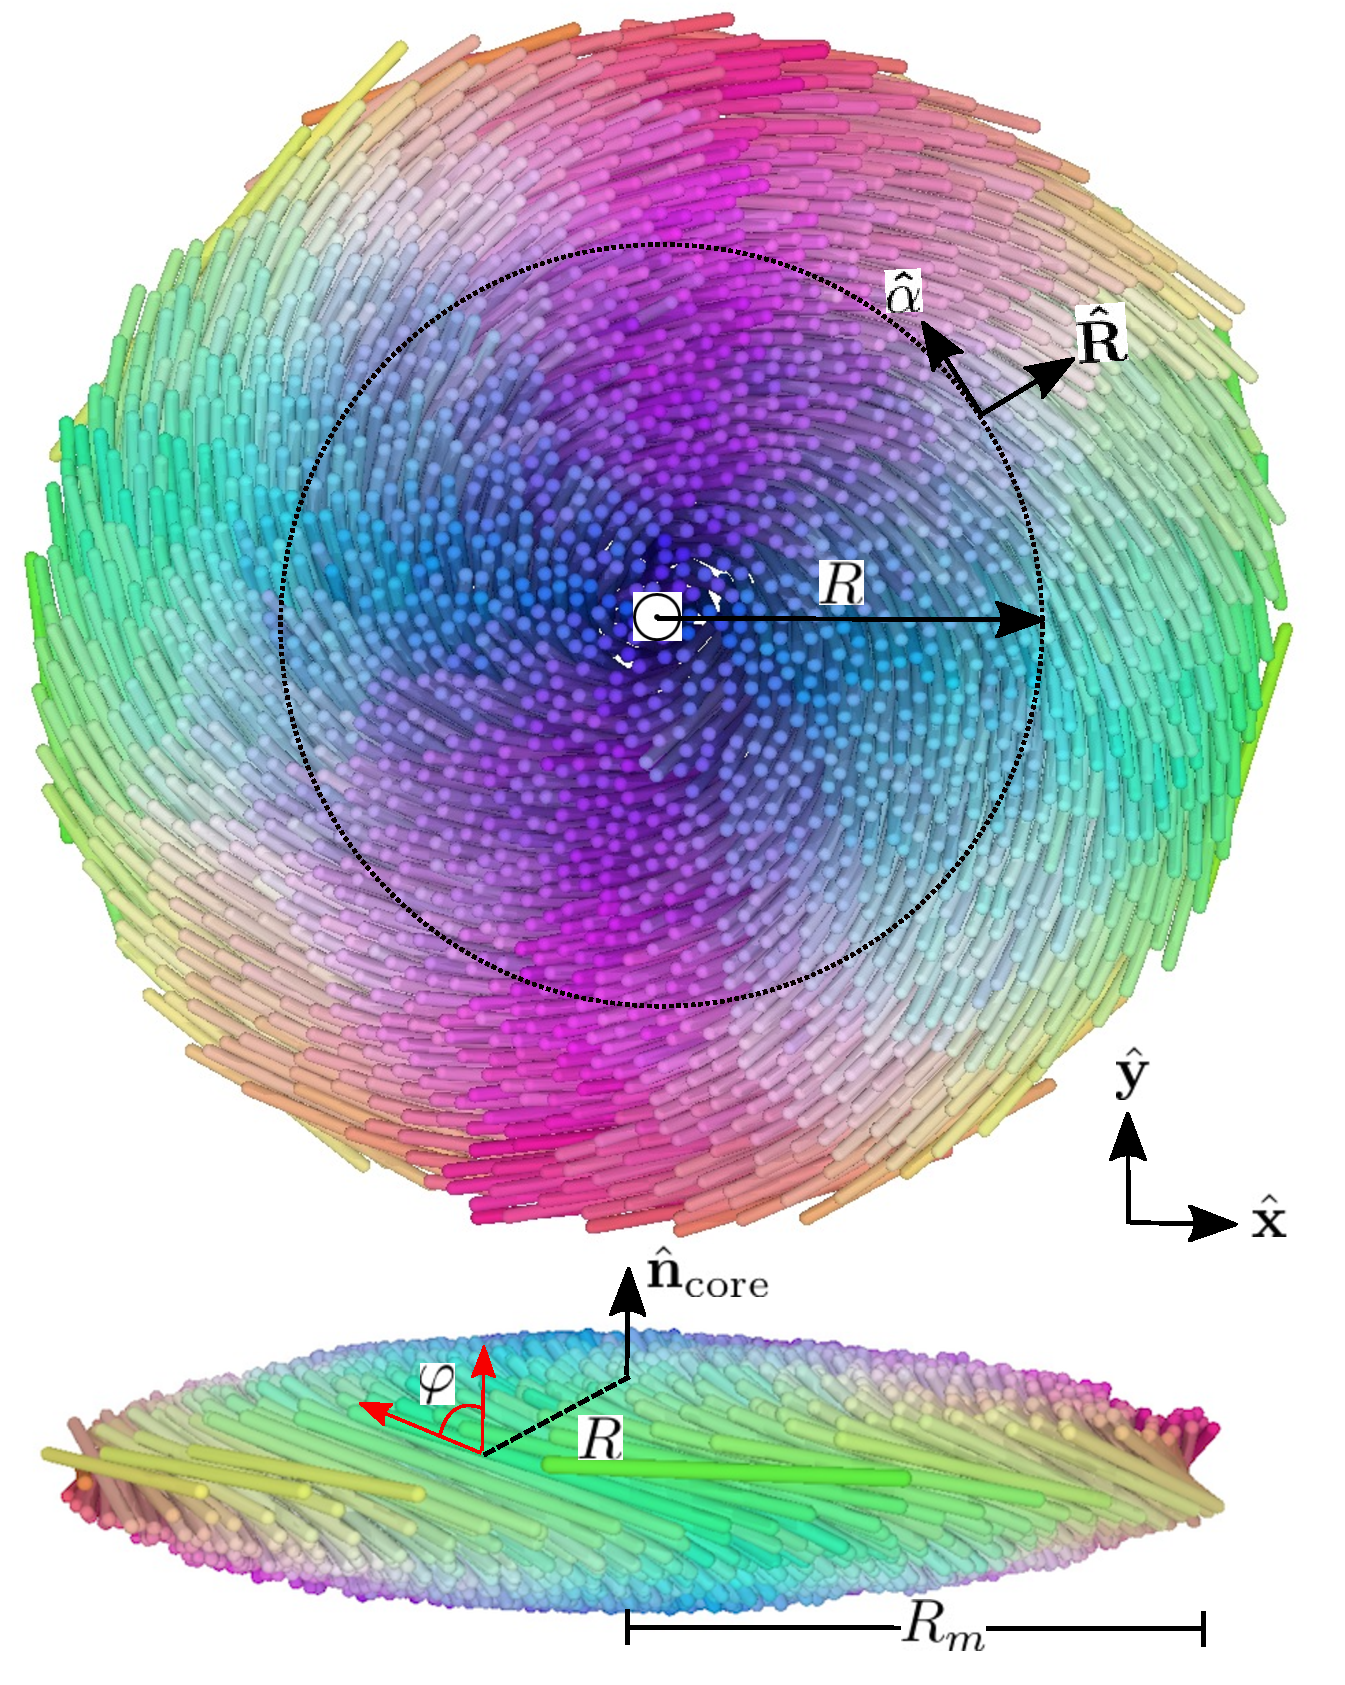
\includegraphics[width= 0.5 \columnwidth]{figures/chapter-5/membranesnapshot}.
\caption{ \label{memsnap} Simulation snapshot of double-twisted smectic membrane of radius $R_{m}$ composed of chiral spherocylinders with aspect ratio $\ell = 20$ mixed with non-adsorbing polymers (not shown) providing strong side-to-side depletion attraction between the rods.  The top graph depict the top view, the lower one a side view of the membrane. The director twist, expressed by the twist angle $\varphi$, is zero at  the membrane  core $\bn _{\rm core} = \bz$ and increases concentrically with radius $R$. Picture courtesy of A. Kuhnhold (Freiburg University, Germany). }
\end{center}
\end{figure}


In an earlier version of our theory \cite{wensink2018elastic} the effect of depletion attraction due to the non-adsorbing polymer can be described in terms of a simple free energy 
\beq
F_{dep}  \sim U_{0} \int d \brr  (\sin \varphi )^{2}  + {\rm cst}
\eeq
where $U_{0}$ is a tilt energy density (per unit area) related to the osmotic pressure of the polymer reservoir and polymer radius of gyration. The simple sine squared contribution is chosen here for simplicity and is in line with de Gennes' original treatment of twist expulsion towards the edges or around defects of smectic layers in analogy with superconductors \cite{gennes-prost, barry_jpcb2009}. It captures the basic trend that the local director tilting away from the membrane normal compromises the free volume experienced by the non-adsorbing polymer  thereby inducing a free energy penalty. In our theory, out-of-plane fluctuations of the rod centre-of-mass away from the 2D plane are not included, but this can be done so on a simple mean-field level \cite{kang_sm2016}.
Ignoring the curvature terms  $R \rightarrow \infty $ and considering a smectic layer on an infinite half-plane enables an analytical minimisation of the free energy in terms of the twist penetration depth $\lambda_{t}  =  \sqrt{K_{2}/a} $ \cite{gennes-prost,barry_jpcb2009}. For the circular membrane, a simple simulated-annealing Monte Carlo algorithm can be employed to minimise the free energy with respect to the twist angle $\varphi(R)$ for any given triplet of length scales, namely the bulk cholesteric pitch $q_{0}^{-1} $, twist penetration depth $\lambda_{t} $ and membrane radius $R_{m}$. With the twist elastic modulus and chiral amplitude being microscopically defined \eq{kexp} a simple one-parameter fitting procedure can be used to determine the depletion strength $a$ and the twist penetration depth $\lambda_{t}$. 



 The main features we established from the numerical results \cite{wensink2018elastic} are the following:  (i) the twisting becomes more pronounced toward the membrane edge when the twist penetration depth becomes shorter, as expected,  but also when membrane size grows larger. (ii) Increasing the pitch $q_{0}$  enhances the maximum twist angle while keeping the overall shape of the twist angle profile largely unchanged. (iii) The local splay angle remains negligibly small  across the membrane so that the omission of splay effects seems fully justified.




\subsection{Scaling results for the elastic moduli for fluid rod membrane}

Using second-virial theory combined with a Gaussian approximation for the orientation probability of the rods within the membrane one can estimate the leading-order contributions of the torque-field, splay, twist and bend elastic constants of a membrane, respectively:
\begin{align}
  K_{1}   & \sim  \frac{17 \rho_{0} \ell^{2}}{24} = \frac{17}{2} K_{2}   \nonumber \\ 
 K_{2}  & \sim  \frac{\rho_{0} \ell^{2}}{12}   \nonumber \\ 
 K_{3} &\sim  \frac{1}{4} K_{2}
  \label{kexp}
\end{align}
Note that the membrane moduli have unity ${\rm N \cdot m}$ (the 3D moduli would be expressed in Newtons) and $\rho_{0} = ND^{2}/A$ refers to planar density of rods with diameter $D$, aspect ratio $\ell = L/D$ and membrane area $A$. The results suggest that the moduli of rodlike particle confined to a membrane are quite different from those of of 3D bulk nematic fluid, at least for strongly elaongated rods experiencing strong nematic order.  In the limit of asymptotic alignment, the splay-to-twist ratio of a bulk fluid  \cite{odijkelastic}  was predicted to scale as $K_{1}/K_{2} \sim 3 $ whereas a much higher ratio $K_{1}/K_{2} \sim 17/2$ is found for the membrane. The bend-to-twist ratio for a hard rod nematic fluid was found to be proportional to the degree of nematic alignment $K_{3}/K_{2} \sim \sigma \gg 1$ \cite{odijkelastic} where $\sigma$ is steered by the rod concentration.  The curvature-to-twist elasticity of a membrane turns out to be smaller than unity $K_{3}/K_{2} \sim 1/4$ and independent of the rod concentration.  In other words, rods confined to a membrane experience a much stronger resistance to splay fluctuations whereas  bend fluctuations are far less penalised compared to a 3D nematic fluid.  Since the splay modulus is about an order of magnitude larger than the twist elasticity, we expect director deformations whereby rods tilt along the radial vector of the membrane to be of marginal importance and  will  be ignored.  





\subsection{Chiral twisting strength }

The pitch $q_{0}$ of a double-twisted membrane can be estimated by considering a weakly chiral pair potential $U_{c}$ described by some arbitrary but short-ranged spatial decay function $g(r)$ describing the range over which chiral forces interact and chiral amplitude $\varepsilon_{c} $ much smaller than the thermal energy. This potential takes the following generic form \cite{goossens1971}:
\beq
U_{c} \sim  \varepsilon_{c} g( r)(\bwa \times \bwb \cdot   \bx) (\bwa \cdot \bwb)
\label{uchi}
\eeq
From this, we may compute the so-called torque-field constant exerted by the chiral potential \cite{wensink2018elastic}:
\beq
K_{t}   \sim -\rho_{0}^{2}  \bar{\varepsilon}_{c} 
\eeq
in terms of an integrated chiral amplitude  $\bar{\varepsilon}_{c}$ which is  {\em different} from that of a  3D cholesteric system as it implicitly encodes the geometric confinement given that $\bdr$ is a 2D vector:
\beq
 \bar{\varepsilon}_{c}  =  \varepsilon_{c} \int d \bdr ( \bdr \cdot \bx)   g( r)
 \eeq
 which has units energy times volume ($k_{B}T \times D^{3}$). From this we find an expression for the typical equilibrium  pitch of the membrane $q_{0} = K_{t}/K_{2}$ that further depends on the in-plane rod density $\rho_{0}$ and rod aspect ratio $\ell = L/D$:
 \beq
 q_{0} \sim \frac{\rho_{0} \bar{\varepsilon_{c}}}{12 \ell^{2}}
 \eeq
The chiral potential drives the twisting of the membrane and $K_{t}$  provides an explicit link between the effective torque-field and the range and amplitude  of the chiral pair potential between a pair of  rods. We remark that the above mean-field treatment will be less adequate for strongly chiral amplitudes $\varepsilon_{c} \gg k_{B}T$. A common choice for $g(r)$ is a short-ranged power law $g(r) = 1/r^{7}$, which is the one we used in our simulations, but  long-ranged forms such as a square-well (SW) potential could be conceivable as well \cite{wensinkjackson}. 


\subsection{Effect of depletants and twist penetration length}

Kang et al. \cite{kang_sm2016} have proposed a more sophisticated expression for the effect of the depletion attraction on the twist angle via the local membrane height $h = (L/2) \cos \varphi$: 
\begin{align}
F_{dep}  \sim & 2 n_{p} a k_{B}T \left [ \int  d {\bf R} \sqrt{ 1 + (\nabla h)^{2} } + \oint d {\bf l} h \right ]
\label{fdep1}
\end{align}
with $n_{p}$ the polymer reservoir pressure and $a$ the polymer radius of gyration. The last contribution is identified a line tension generated by depletion forces between rods. Combining this with the elastic part of the 
\eq{fmem} we find the following free energy for a membrane with radius $R_{m}$:
\begin{align}
\frac{ F}{K_{2}}  &\sim \int  d \brr   \left [  \left ( \partial_{R} \varphi + \frac{\sin 2 \varphi}{2R} + q_{0} \right )^{2}  + \frac{K_{3}}{K_{2}}\frac{ ( \sin \varphi )^{4}}{R^{2}} \right . \nonumber \\ 
& \left .  + \lambda_{t}^{-2}    \sqrt{ 1 + (\partial_{R} h)^{2} }   \right ]  + 2 \pi  \lambda_{t}^{-2} R_{m} h(R_{m})
\label{fmem1}
\end{align}
with $\int d {\bf R} = 2 \pi \int_{0}^{R_{m}} R dR $ in circular coordinates. The line tension contribution drops with increasing twist at the edges and  becomes zero if the rods are twisted perpendicular to the membrane normal $\phi(R_{m} = \pi/2)$. 
The twist penetration length is given by $\lambda_{t} = \sqrt{K_{2}/2  n_{p} a k_{B}T}$ which, using \eq{kexp} leads to a compact expression depending on quantities known from experiment such as the in-plane rod density (assumed uniform across the membrane), rod-polymer size ratio $D/a$, rod aspect ratio $\ell$ and the reservoir polymer concentration $n_{p}$: 
\beq
\frac{\lambda_{t}}{D} = \sqrt{\frac{\rho_{0} \ell^{2} }{24  (n_{p} a^{3}) (D/a)^{2} }}
\eeq
Taking typical numbers from our simulation ($\ell \sim 10$, $\rho_{0} \sim 0.5$, $D/a=2$ and $n_{p}a^{3} \sim 0.2$) we find that that the twist penetration length is only a few times the rod diameter, i.e. $\lambda_{t} \sim 2 D$. 
For {\em fd} rods a much larger value is found primarily because they are longer than our rods ($\ell \sim 130$). The predicted value $\lambda_{t} \sim 20 D$ is roughly line with the experimentally measured value of about half a rod length   depending on the polymer concentration that was used to stabilize the membranes \cite{barry_jpcb2009}.

In Ref. \cite{kuhnhold2022colloidal} a simple trial form was used to fit the simulation data:
\beq
\varphi(R) = \varphi_{0} \left ( \frac{R}{R_{m}} \right )^{\alpha} 
\eeq
with $\varphi_{0}$ the twist angle at the membrane edge and $\alpha $ a variational parameter governing the degree of twist near the edge.  It is tempting to insert the trial form into the free energy \eq{fmem1} and seek an algebraic minimization route through the variational parameters $\varphi_{0}$ and $\alpha$.   However, such an approach turns out to be too unfeasible because the free energy is strongly non-linear in $\varphi$.  As in Ref. \cite{wensink2018elastic} we therefore employ a simulated-annealing Monte Carlo algorithm to obtain the angular profile as a function of the distance from the membrane core. 

\section{Starfish instability and twisted ribbon}

At elevated chiral strength the circular membranes are known to transition into twisted ribbons \cite{Gibaud2014}. These were identified as quasi-1D twisted protrusions growing out of the perimeter of the membrane, through a mechanism termed `starfish' instability. 


Lowering the temperature strengthens the chiral forces between  rods which raises the free energy of interior untwisted rods while lowering the free energy of edge-bound twisted rods. This enables chiral control of edge line tension which, when the edge tension approaches zero,  leads to spontaneously transitions of the membrane into an array of 1D twisted ribbons, called a ‘‘starfish’’ \cite{Gibaud2014}.


We may adopt the same reasoning as before and formulate a free energy for a double-twisted  ribbon. First, the director field of a twisted ribbon may be constructed from a combination of two rotation matrices, each corresponding to a twist along mutually perpendicular Cartesian axes. Without loss of generality we fix the director field of the untwisted ribbon along the $x$-axis of the frame $\bn_{0}=(1,0,0)$ so that the director field of the ribbon reads: 
\beq
\bn_{r}[ \Phi, \chi] = \mathcal{R}_{xz} [\Phi]\cdot \mathcal{R}_{xy}[\chi] \cdot \bn_{0}
\eeq
in terms of the rotation matrices
 \beq
 \mathcal{R}_{xz} [ \Phi]   =
  \begin{bmatrix}
     \cos \Phi(y) & 0 & \sin \Phi(y)  \\
    0 & 1 & 0  \\
    -\sin \Phi(y) &  0 & \cos \Phi(y)  \\
      \end{bmatrix}  \nonumber
      \label{rxz}
 \eeq
and
 \beq
 \mathcal{R}_{xy} [ \chi]   =
  \begin{bmatrix}
     \cos \chi(z) &  \sin \chi(z) & 0  \\
    -\sin \chi(z) &   \cos \chi(z) & 0 \\
      0 & 0 & 1  \\
      \end{bmatrix}  \nonumber
      \label{rxy}
 \eeq
Here, $\Phi$ and $\chi$ denote  two  angles describing the twist along the short and long (ribbon) axes that we parameterize via the coordinates $0 < y < s_{y}$ and $0< z <s_{z}$, respectively. The ribbon area $A = s_{y}s_{z}$ is conserved. We further define the local thickness of the ribbon:
\begin{align}
h = \frac{L}{2}   | \bn_{0} \cdot \bn |  =\frac{L}{2} |\cos \chi(y) \cos \Phi(y)| 
\end{align}
We now simplify matters by assuming linear twist in both directions so that $\Phi = qy$ and $\chi = q \gamma z$ in terms of a pitch $q$ which does not necessarily coincide with the pitch $q_{0}$ defined for the double-twisted membrane as we shall see later. Furthermore, $\gamma$ denotes a {\em twist anisotropy} which is unequal to one if the twist along the short and long ribbon axes is not the same. Both $q$ and $\gamma$ will be determined from the minimum conditions for the total free energy of the ribbon. We will ignore any twist anisotropy and simply fix $\gamma =1$  for the moment. Next, assuming weak twist on the scale of the rod diameter $q \ll D^{-1}$ we Taylor expand for $q$ and keep the leading-order term of the  bulk (Frank) elastic energy of the ribbon which turns out to be of quartic order:
\beq
\frac{F_{bulk}}{A} \sim  \frac{1}{24} \left [  K_{3} q^{4}(s_{y}^{2} + s_{z}^{2}) +   K_{2} q_{0} q^{3}(2s_{y}^{2} - s_{z}^{2})  \right ]  + \mathcal{O}(q_{0}^{6})
\eeq
The depletion  contribution \eq{fdep1} can be derived in a similar way. 
Straighforward algebra then gives up to leading order:
\begin{align}
\frac{F_{dep}}{A}  & \sim  2 n_{p} a k_{B}T \left [1 + \frac{q^{4}L^{2}}{96}(s_{y}^{2} + s_{z}^{2})  + A^{-1} \oint d {\bf l} h \right ]
\end{align}
Twisting a rectangular slab into a ribbon enhances the contour length of the object which is reflected in the line integral in \eq{fdep1} that we express as $\oint d {\bf l}h = \sqrt{1+ (q s_{y}/2)^{2}}\int_{0}^{s_{z}} dz h$. Expanding the ribbon perimeter up to quartic order in $q$ we write:
\beq
 \oint d {\bf l} h  \sim L [ w_{0} + w_{2} q^{2} + w_{4} q^{4} ]
\eeq
The coefficients depend only on the ribbon dimensions and will be specified shortly.
The leading order contribution of the  does not depend on the degree of twist. 
Finally we consider the effect of saddle-splay which is non-zero due to the curvature of the ribbon (it does not play a role for the flat membranes). It can be defined as a the following bulk contribution to the Frank elastic energy: 
\beq
F_{se} = -\frac{K_{24}}{2} \int d \bfr   [\nabla \cdot ( \bn \nabla \cdot \bn +  \bn \times \nabla \times \bn )]
\eeq
which gives within our approximation:
\beq
\frac{F_{se}}{A} \sim -\frac{q^{4}}{24} K_{24}  (s_{y}^{2} + s_{z}^{2}) 
\eeq
Combining terms and reintroducing the twist penetration length $\lambda_{t}$ we arrive at a compact expression for the total free energy of a twisted ribbon:
\begin{align}
\frac{F}{AK_{2}} &\sim  \frac{1}{24} \left [ \Delta K q^{4} (s_{y}^{2} + s_{z}^{2}) +  q_{0}q^{3} (2s_{y}^{2} - s_{z}^{2})  \right ] \nonumber \\ 
& + \frac{L }{ A \lambda_{t}^{2}} [ w_{0} + w_{2} q^{2} + w_{4} q^{4} ]
\end{align}
in terms of the  constant
\beq
\Delta K = (L/2\lambda_{t})^{2} +  (K_{3} - K_{24})/K_{2}
\label{dk}
\eeq
It is expedient at this stage to render the free energy and pitch dimensionless  by renormalizing in terms of the short ribbon edge $s_{y}$ via $F \rightarrow F s_{y}^{2} /K_{2}A = F/K_{2}\tau$ and $q \rightarrow   qs_{y}$ in terms of  the {\em ribbon aspect ratio} $\tau = s_{z}/s_{y}$. Ignoring all constant factors  we  find a much more manageable expression:
\begin{align}
\frac{F}{K_{2}} & \sim  \frac{1}{24} \tau \left [ \Delta K q^{4} (1 + \tau^{2}) +   q_{0}q^{3}(2-\tau^{2})  \right ] \nonumber \\ 
& + \Delta \ell [ w_{0} + w_{2} q^{2} + w_{4} q^{4} ]
\label{fribbon}
\end{align}
with $\Delta \ell = Ls_{y} / \lambda_{t}^{2} $ denoting an effective surface tension. 
The coefficients appearing in the last term related to the line tension only depend on the ribbon aspect ratio and are as follows:
\begin{align}
w_{0} &= (1 + \tau)  \nonumber \\ 
w_{2} &= -\frac{1}{24}  (1 + 3 \tau^{2} + \tau^{3} ) \nonumber \\
w_{4} &=  \frac{1}{1920} (1 - 40 \tau + 10 \tau^{2} + 5 \tau^{4} + \tau^{5})
\end{align}
Before proceeding with our analysis we immediately infer a couple of basic facts from inspecting \eq{fribbon}. First, as expected chiral forces between the rods, represented by the term proportional to $2-\tau^{2}$, lower the free energy provided the ribbons are sufficiently elongated ($\tau  >\sqrt{2})$. A further stabilization mechanism occurs through the line tension since the curvature correction $w_{2}$ is negative. This reflects the phenomenon that chiral twist reduces the line tension of the droplet which subsequently powers various morphological changes, in particular the membrane-starfish transition reported in Ref. \cite{Gibaud2014}. 

The relevant constants $\Delta K$ and $\Delta \ell$ can be estimated from the twist penetration length. Taking the reference value $\lambda_{t} = L/2$ quoted for {\em fd} virus rods we find that  $\Delta K \sim (L/2\lambda_{t})^{2} \sim 1 $,  ignoring weak contributions from the bend-to-twist and saddle-splay elasticity. Similarly, we obtain $\Delta \ell \approx 4 $ for a ribbon with a lateral width equal to the rod length $s_{y} = L$. For the pitch we roughly estimate $q_{0} = 2 \pi s_{y} / p_{c} \approx 0.2$ taking a cholesteric pitch  $p_{c} \sim 30L$. 

The next step is to minimize the free energy \eq{fribbon} with respect to the ribbon pitch $q$ and aspect ratio $\tau$, i.e., $\partial F/\partial q =0$ and $\partial F/\partial \tau =0$ for a given ribbon area $A$. If the line tension is ignored ($\Delta \ell =0$), the extremum condition can be solved analytically and gives an equilibrium ribbon pitch:
\beq
q =  \frac{3q_{0}}{4 \Delta K} \frac{(\tau^{2} -2)}{1 + \tau^{2}}
\eeq
where the last contribution is a monotonically increasing function for $\tau^{2} >2$ levelling off to unity for $\tau \gg 1$. The ribbon free energy per unit area corresponding to the optimal pitch is:
\beq
\frac{F/\tau}{K_{2}}  = -\frac{1}{96} q_{0}  (\tau^{2} -2) q^{3}
\eeq
From this we infer that (i) stable ribbons that are not curbed by line tension penalty tend to stretch to very large aspect ratios, and (ii) the limiting pitch at large ribbon aspect ratio is likely smaller than the membrane pitch $q_{0}$ given that $q =  3q_{0}/4 \Delta K$ for $\tau \rightarrow \infty $ and $\Delta K \sim 1$.

In practice, conservation of area precludes the ribbons to stretch to infinity while a finite line tension puts a further natural bound to $\tau$. 


\subsection{Effect of anisotropic twist} 


\begin{figure}
\begin{center}
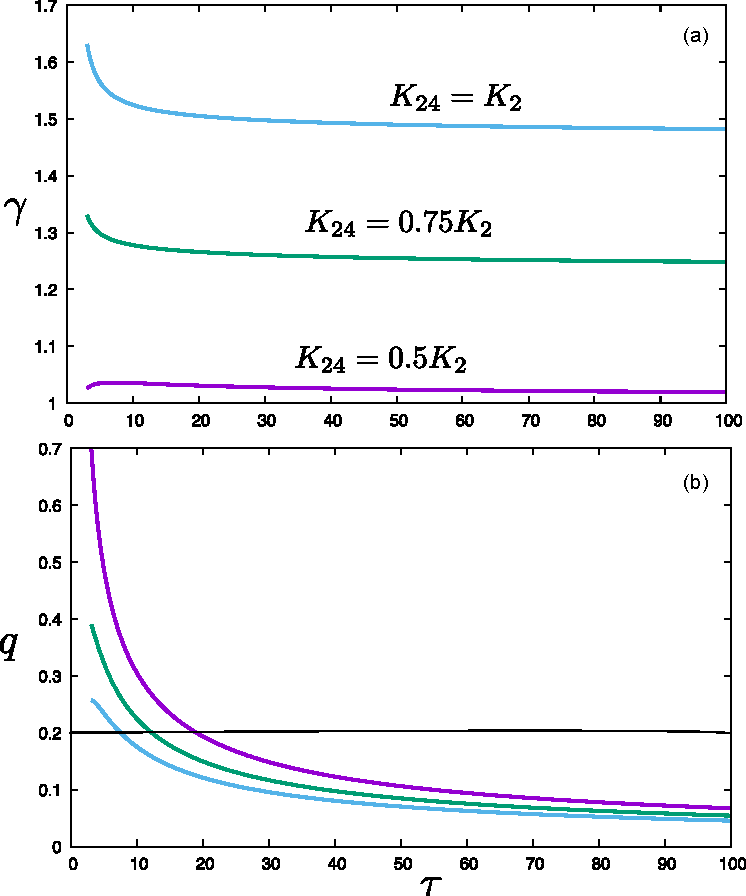
\includegraphics[width=  0.5 \columnwidth]{figures/chapter-5/raniso}.
\caption{ \label{fig3} Twist anisotropic $\gamma$ and pitch $q$ of a twisted ribbon as a function of the ribbon aspect ratio $\tau$. The chiral strength between the rods is given by the membrane pitch $q_{0} = 0.2$ (horizontal black line). The twist penetration length is $\lambda_{t} = 0.5 L$.   }
\end{center}
\end{figure}


Let us now explore the possibility of unequal twist along the short and long ribbon axes. This should render a more realistic picture of the internal twist profile of the ribbon  given that the twist along the principal ribbon directions need not have the same magnitude. We proceed by allowing $\gamma$, which denotes the ratio between the degree of twist along the long and short axes  of the ribbon,  to be a  variable quantity. Working out the algebraic free energy per area we find for the bulk elastic contribution:
\begin{align}
\frac{F}{ K_{2} \tau} &\sim 
\frac{1}{24} \left [ \frac{K_{3}}{K_{2}} q^{4} (1 + \tau^{2}) \gamma^{2} + B\right ]
\end{align}
with $B$ the twist elastic contribution:
\beq
B = (q_{0} + q - q \gamma) (12 q_{0} + q (12 - \gamma (12 + q^2 ( \tau^{2} \gamma -2))))
\eeq
This term reduces to the much simpler expression explored in the previous section for the isotropic twist case ($\gamma =1$). Similarly, the saddle-splay term now becomes:
\beq
 \frac{F}{K_{2} \tau} \sim  - \frac{1}{24}\frac{K_{24}}{ K_{2} } q^{4} \gamma (1 + \tau^{2} \gamma)
\eeq
Finally the depletion free energy reads (ignoring irrelevant constants as well as the line tension contribution):
\beq
 \frac{F}{K_{2} \tau} \sim  \frac{L^{2}}{96 \lambda_{t}^{2}} q^{4} (1 + \tau^{2} \gamma^{4})
\eeq
Clearly, these complex expressions are no longer amenable to further analytical treatment. Furthermore, the elastic and depletion strengths can longer be compactly combined into a  single parameter $\eq{dk}$ as could be done for the isotropic twist case but must be  separately defined. However, minimization of the three free energy terms above with respect to $q$ and $\gamma$ is easily carried out numerically and the results are shown in \fig{fig3} taking $K_{3}/K_{2} = 1/4$, $q_{0} = 0.2$, $\lambda_{t} = L/2$ and three different values for the saddle-splay elastic modulus. Clearly,  $\gamma $ tends to be larger than unity depending on the strength of the saddle-splay elasticity $K_{24}$ indicating twisting along the main ribbon axis can be about 30-50 \% stronger than across the short axis. We remark that $K_{24}$ plays an essential role in driving the double twist for the ribbon geometry. In fact, saddle-splay elasticity cannot be ignored given that  no physical solutions of the minmization problem were found  for $K_{24} =0$. The lowest value explored ($K_{24} = K_{2}/2$) roughly recovers the previous scenario of equal twist along the short and long ribbon axes.  We further conclude from \fig{fig3}b that longer ribbons tend to be less twisted than short ones.   Short ribbons ($\tau <10$) seem {\em overtwisted} compared to that of the equivalent (single twist) cholesteric phase while long ribbons experience less twist. In all cases we see that $q$ levels off to a limiting value $q < q_{0}$ for infinitely stretched ribbons ($\tau \rightarrow \infty$) in line with our analytical predictions for the case of constrained isotropic twist $\gamma =1$. The line tension, ignored in the results of \fig{fig3}, will put a constraint on the optimal aspect ratio $\tau$ which needs to optimized along with $q$ and $\gamma$ for a given ribbon area. We will not pursue this further in this study given that, in experiment, the line tension at the starfish transition is very low while the available virus material and hence the area tends to be quite large. Both  factors enable these ribbons to grow into strongly elongated objects. This should be compared to our predictions for the limiting case $\tau \rightarrow \infty$. Further restriction  to applying our model to experiments relates to the unknown saddle-splay constant for {\em fd} virus rods. 







\clearpage